\documentclass{article}
\usepackage[utf8]{inputenc} %cp1252 pour Windows, utf8 pour Linux
\usepackage[T1]{fontenc}
\usepackage{lmodern}
\usepackage{graphicx}
\usepackage[frenchb]{babel}
\usepackage{hyperref}
\usepackage[table,xcdraw]{xcolor}
\usepackage{float}

\newcommand{\info}{\texttt}
\newcommand{\qt}{\info{QuadTree}}

\title{Algorithmique et Structure de Données 2\\
	Rapport Projet 2}
\author{Valentin \bsc{Hénique} \and Corentin \bsc{Chédotal}}
\date{02 Mai 2016}

\begin{document}
	
	\maketitle
	
	\section{Introduction}
	
	Dans le cadre de l'Unité d'Enseignement X4I0030 intitulée "Algorithmique et Structure de Données 2" nous avons été amené à produire un second et dernier projet. Celui-ci consiste en la réalisation d'un algorithme de compression d'images bitmap. Pour ce faire nous avions à notre disposition un arbre de recherche d'arité 4 : le \qt. Il était donc demandé de représenter les images à travers ces arbres particuliers en suivant une méthode spécifique expliquée dans le sujet. Ceci fait il nous fallait appliquer nos algorithmes de compressions et comparer divers réglages de ceux-ci.
	Le langage de programmation demandé étant le C++.\\
	Ce rapport expliquera donc comment ces algorithmes ont été mis en place ainsi que les contraintes mémorielles et temporaires de ceux-ci. Nous comparerons d'ailleurs différents fonctionnements de ceux-ci dans des environnements de test spécifiques qui eux aussi seront expliqués.
	
	\section{Implémentation}
	
	Afin de répondre aux exigences du sujet plusieurs décisions concernant l'implémentation ont été prises. Tout d'abord comme demandé l'encodage des images se fait initialement par l'intermédiaire de la structure ImagePNG puis le stockage se fait dans la structure arbre d'arité 4 \qt\ telle que présentée dans le sujet et donnée dans la bibliothèque fournie. C'est dans cette structure que les éventuelles opérations de compression (sans-perte, delta ou phi) sont effectuées. Il a aussi été décidé que pour les méthodes nécessitant de travailler sur l'arbre une approche récursive serait la plus appropriée et donc les méthodes publiques font souvent appel à des méthodes privées dont le fonctionnement est récursif. Le but de cette pseudo-duplication des méthodes était de ne pas changer les méthodes publiques par rapport à celles données de base à l'exercice tout en ayant la possibilité de faire ce fonctionnement récursif qui nécessitait des paramètres supplémentaires.\\
	Enfin la liste de toutes les méthodes employées est explicitée ci-après.
	
	\subsection{Méthodes employées}
	
	\subsubsection{Méthodes publiques}
	
	\begin{itemize}
		\item \info{QuadTree()} : Constructeur initialisant un arbre d'arité 4 vide.
		\item \info{~QuadTree()} : Destructeur faisant appel à la méthode \info{destructeur()} sur la racine du \qt.
		\item \info{afficher()} : Méthode d'affichage textuel du contenu d'un \qt\, appelle la méthode \info{afficher\_rec()} sur la racine dans le cas d'un arbre non vide. Présente à des fins de debugging.
		\item \info{importer(const ImagePNG \& img)} : Encode l'image Bitmap img (au format ImagePNG) dans le \qt. Emploie la méthode \info{importer\_rec()}. L'image doit être de dimension $2\up{n}\times2\up{n}$ avec $n>0$.
		\item \info{exporter()} : Méthode exportant le contenu du \qt\ dans une image sous le format ImagePNG. Fait appel au constructeur d'ImagePNG et à \info{exporter\_rec()}.
		\item \info{compressionDelta(unsigned delta)} : Méthode de compression d'un \qt\ et donc de son image associée basée sur un seuil maximal de différence en luminance entre les pixels. Ici delta est le seuil choisi pour la compression. Etant donné les limites des couleurs des pixels on a $delta<255$. Emploie ou \info{compressionSansPerte\_rec()} ou \info{compressionDelta\_rec} suivant la valeur de delta.
		\item \info{compressionPhi(unsigned phi)} : Autre méthode de compression d'un \qt\ et de l'image encodée dans celui-ci. Celle-ci est basée sur un nombre maximal de feuilles restant après la compression. Ce nombre est le paramètre phi, or la compression ne pouvant aps supprimer le \qt\ dans son intégralité on a $phi>0$. Fais appel aux méthodes privées \info{destructeur()} et info{stockLumMax()}.
	\end{itemize}
	
	\subsubsection{Méthodes facilitatrices (privées)}
	
	\begin{itemize}
		\item \info{kiemeBit(unsigned n, unsigned k)} : Méthode statique simple retournant la valeur du k-ième bit d'un entier n positif. Présente afin de simplifier les calculs.
		\item \info{afficher\_rec(const Noeud * n, std::string tabs="")} : Méthode d'affichage textuel du \qt\ de façon récursive. Le paramètre n est le noeud duquel l'affichage se fait en "descendant".
		\item \info{destructeur(Noeud * ptr)} : Méthode détruisant les nœuds et feuilles "plus bas" que ptr de façon récursive. Permet donc des destructions "sélectives" ou un emploi général depuis la racine comme destructeur du \qt\ entier.
		\item \info{importer\_rec(Noeud * ptr, unsigned taille, const ImagePNG \& img, unsigned x, unsigned y)} : Méthode créant le \qt\ à partir d'une image de façon récursive en "descendant" et construisant l'arbre petit à petit, le remplissant des valeurs des pixels au fur et à mesure. Ici ptr est le noeud à partir duquel on descend pour contruire les feuilles suivantes, taille est la largeur de l'image, image est l'image au format ImagePNG à encoder dans le \qt\ et x et y sont les positions en cours afin de placer correctement les pixels aux bons endroits de l'arbre. L'image doit par contre être au format $2\up{n}\times2\up{n}$ avec $n>0$.
		\item \info{exporter\_rec(const Noeud* ptr, unsigned taille, ImagePNG \& img, unsigned x, unsigned y)} : Méthode créant une image au format ImagePNG depuis les valeurs des pixels encodés dans le \qt\ de façon récursive. Fonctionne de la même façon que plus haut mais ici on va extraire les valeurs des feuilles de l'arbre afin de les mettre dans les pixels correspondant de image. A nouveau l'image doit être au format $2\up{n}\times2\up{n}$ avec $n>0$.
		\item \info{compressionSansPerte\_rec(Noeud* ptr, unsigned taille)} : Algorithme de compression récursif d'une image sans perte (dans le cas d'une compression Delta avec delta=0). Le paramètre ptr est le pointeur vers le Noeud duquel on effectue les éventuelles opérations de compression sur ses feuilles, taille est simplement la largeur de l'image.
		\item \info{compressionDelta\_rec(Noeud* ptr, unsigned taille, unsigned delta)} : Algorithme de compression récursif d'une image avec perte basée sur la différence de luminance des pixels voisins. Le paramètre ptr est le pointeur vers le Noeud duquel on effectue les éventuelles opérations de compression sur ses feuilles, taille est simplement la largeur de l'image et delta est la différence de luminance requise.
		\item \info{stockLumMax(Noeud* n, unsigned taille, std::vector<std::pair<unsigned, Noeud*>> * vecStock)} : Méthode permettant de stocker des pointeurs et leurs luminances associées dans des paires elles même stockées dans un Vector. Le paramètre n est le pointeur du noeud sur lequel les opérations sont effectuées, taille est la largeur de l'image et vecStock est le Vector dans lequel seront stockées les paires.
	\end{itemize}
	
	\subsection{Encombrement mémoire}
	
	Initialement l'encombrement mémoire est maximum. En effet lors de l'importation d'une image il existe autant de feuilles que de pixels plus les nombreux pointeurs des différents nœuds. Une fois l'importation terminée l'encombrement ne varie plus sauf si une opération de compression est lancée sur le \qt. Auquel cas l'encombrement va augmenter un cours instant (le temps de faire le premier calcul de moyenne et de la conservation de celle-ci) puis ne fera que baisser.
	
	\subsection{Complexités temporelles}
	
	Travaillant avec des images pouvant atteindre des tailles particulièrement grandes l'étude de la complexité temporelle des différents algorithmes employés est particulièrement importantes. Il faut pouvoir optimiser au maximum ceux-ci puisque dans le cas des images de plus de huit mille pixels de largeur certaines opérations seront donc effectuées sur plus de soixante-quatre millions de pixels. Nous allons donc fournir ici les complexités théoriques ainsi que divers exemples d'utilisation des \qt\ et les valeurs expérimentales de temps d'exécution.
	
	\subsubsection{Complexités temporelles théoriques}
	
	Ci-dessous se trouve un tableau des complexités temporelles théoriques des diverses méthodes du \qt\ :
	\begin{table}[H]
		\centering
		\label{ComplexiteTheo}
		\begin{tabular}{|l|l|}
			\hline
			\rowcolor[HTML]{C0C0C0} 
			{\color[HTML]{333333} \textbf{Méthodes}} & \textbf{Complexité} \\ \hline
			\info{QuadTree()}                                 &  $\Theta(1)$                   \\ \hline
			\info{\char`\~QuadTree()}                                &  $\Theta(nb de Noeud)$                   \\ \hline
			\info{afficher()}                                &  $O(nb de Noeud)$                   \\ \hline
			\info{importer()}                                 &  $\Theta(nb de Noeud)$                   \\ \hline
			\info{exporter()}                               &  $\Theta(nb de Noeud)$                   \\ \hline
			\info{compressionDelta()}                                &  $\Theta(nb de Noeud)$                   \\ \hline
			\info{compressionPhi()}                                 &  $\Theta(nb de Noeud + taille)$                   \\ \hline
			\info{kiemeBit()}                                 &  $\Theta(1)$                   \\ \hline
			\info{afficher\_rec()}                                 &  $\Theta(nb de Noeud)$                   \\ \hline
			\info{destructeur()}                                 &  $\Theta(nb de Noeud)$                   \\ \hline
			\info{importer\_rec()}                                 &  $\Theta(nb de Noeud)$                   \\ \hline
			\info{exporter\_rec()}                                 &  $\Theta(nb de Noeud)$                   \\ \hline
			\info{compressionSansPerte\_rec()}                                 &  $\Theta(nb de Noeud)$                   \\ \hline
			\info{compressionDelta\_rec()}                                 &  $\Theta(nb de Noeud)$                   \\ \hline
			\info{stockLumMax()}                                 &  $\Theta(nb de Noeud)$                   \\ \hline
		\end{tabular}
		\caption{Complexités Temporelles Théoriques des opérations sur les \qt}
	\end{table}
	
	\subsubsection{Complexités temporelles expérimentales}
	
	Comme les complexités théoriques peuvent ne pas forcément parler autant que des résultats expérimentaux et afin de confirmer le bon fonctionnement des algorithmes la partie qui suit s'intéresse aux complexités temporelles obtenues lors de tests. Cette section ne s'attardera cependant mais uniquement aux résultats mais aussi à la façon de réaliser les tests ainsi que sur le contenu de ces tests et leur pertinence.
	
	\paragraph{Protocole expérimental}
	
	Deux séries de tests ont été effectuées. La première par le biais du Makefile pour une image donnée. En effet le programme va simplement effectué les opérations demandées par l'utilisateur ce qui ce présente d'une certaine façon comme des jeux de tests de l'ensemble des méthodes sur une image donnée (à part évidemment celles de compression qui ne se font qu'une à la fois bien sur). L'image compressée est ensuite produite comme celles présentes dans le répertoire de ce rapport à titre d'exemple.\\
	Deuxièmement de part l'utilisation du fichier Mesure.cpp des mesures du temps d'exécution pour différentes images et compressions ont été faite afin de les comparer aux complexités temporelles théoriques explicitées plus haut.
	
	\paragraph{Base de jeux de test et pertinence de ceux-ci}
	
	Les différentes méthodes d'importation, d'exportation et de compression voyaient leur temps d'exécution mesurés dans un environnement particulier. En effet elles ont été testées pour les images de 128, 512 et 2048 pixels de largeur. Ainsi cela permet de voir l'évolution du temps d'exécution par rapport à une largeur de plus en plus grosse. De plus les mesures de compression ce sont faite avec les même paramètres, une compression delta avec un delta égal à 0 afin de mesurer la compression sans perte, une compression delta avec un delta égal à 50 et une avec delta égal à 200 afin d'avoir une image assez représentative du temps mis par la compression delta suivant sont delta et enfin la même chose pour la compression phi.
	
	\paragraph{Résultats}
	
	Ce faisant on obtient les graphes ci-dessous :
	\begin{figure}[H]
		\begin{center}
			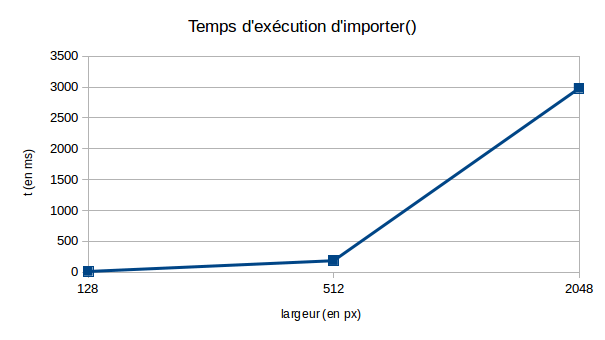
\includegraphics[scale=0.5]{grapheImporter}
			\label{grapheImporter}
		\end{center}
	\end{figure}
	\begin{figure}[H]
		\begin{center}
			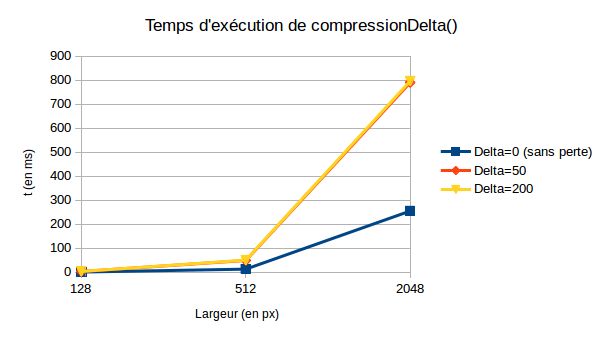
\includegraphics[scale=0.5]{grapheCompressionDelta}
			\label{grapheCompressionDelta}
		\end{center}
	\end{figure}
	\begin{figure}[H]
		\begin{center}
			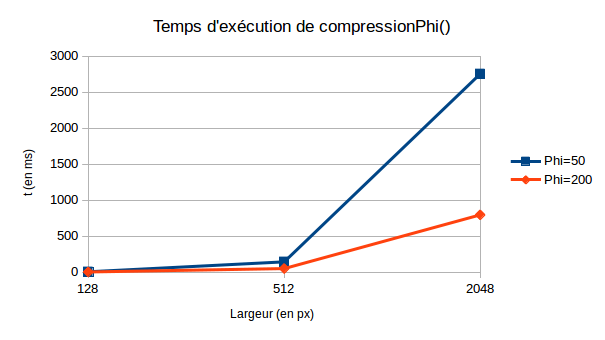
\includegraphics[scale=0.5]{grapheCompressionPhi}
			\label{grapheCompressionPhi}
		\end{center}
	\end{figure}
	\begin{figure}[H]
		\begin{center}
			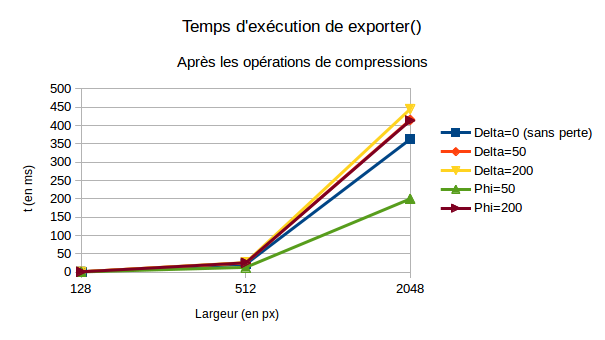
\includegraphics[scale=0.5]{grapheExporter}
			\label{grapheExporter}
		\end{center}
	\end{figure}
	Ces résultats étayent nos représentations théoriques du fonctionnement des diverses méthodes invoquées. De plus ils font apparaître la raison pour laquelle nous n'avons pas pu effectuer de mesures sur les images les plus volumineuses. En effet lors de nos essais il s'est révélé que les ordinateurs de la faculté comme les ordinateurs portables que nous utilisons pour les cours et qui s'avèrent ancien n'arrivaient pas à faire tourner complètement les algorithmes sur les images plus grosses. Ces graphes font effectivement apparaître la vitesse à laquelle les temps augmentent et à cela comme expliquer précédemment il faut ajouter l'encombrement de la mémoire vive.
	
	\section{Conclusion}
	
	En conclusion ce projet fut relativement difficile mais le temps donné était approprié. En effet nous n'avons jamais ressenti le fait d'être pressé par le temps mais par contre la réalisation du sujet demandé fut ardue. La compréhension du sujet d'abord requerra toute une séance de brainstorming et obligeait après des périodes un peu trop longues sans toucher au sujet un temps de ré-acclimatation assez long. A cela s'ajoutait l'utilisation d'une bibliothèque encore inconnue et qui n'était pas inclue de base dans les distributions du C++ et tous les problèmes qui pouvaient aller avec. Enfin la mise en oeuvre du \qt\ était un peu particulière comme tout déplacement devait être fait par récursivité afin d'être optimal à celle-ci il fallait ajouter les opérations de compression qui nécessitaient donc de garder à la fois une vision d'ensemble du \qt\ et de l'image en tant que telle mais aussi des calculs à faire à chaque niveau, que ce soit des noeuds ou des feuilles. Or ceux-ci éaient liés à des pointeurs nécessitant donc une grande prudence afin d'éviter les erreurs de segmentation mais aussi et surtout les fuites mémoires.\\
	Ceci dit tout pu être fait dans les temps et les questions d'optimisation du code ayant été évoquées dès la conception de celui-ci la phase d'optimisation en tant que telle fut assez courte. Ce fut un projet enrichissant car finalement très pratique puisque l'on a un résultats finalement très visible de notre travail avec les images compressées.
	
	\newpage
	\tableofcontents
	
\end{document}
